\section{Discrete convex geometry by examples}\label{Examples}

\subsection{Terminology}\label{Term}

For the precise interpretation of parts of the Normaliz output some terminology is necessary, but this section can be skipped at first reading, and the user can come back to it when it becomes necessary. We will give less formal descriptions along the way. The following applies to rational polyhedra. Algebraic polyhedra are discussed in Section~\ref{Algebraic}.

As pointed out in the introduction, Normaliz ``computes'' intersections $P\cap L$ where $P$ is a rational polyhedron in $\RR^d$ and $L$ is an affine sublattice of $\ZZ^d$. It proceeds as follows:

\begin{arab}
	\item If the input is inhomogeneous, then it is homogenized by introducing a homogenizing coordinate: the polyhedron $P$ is replaced by the cone $C(P)$: it is the closure of $\RR_+(P\times \{1\})$ in $\RR^{d+1}$. Similarly $L$ is replaced by $\widetilde L=\ZZ(L\times \{1\})$. In the homogeneous case in which $P$ is a cone and $L$ is a subgroup of $\ZZ^d$, we set $C(P)=P$ and $\widetilde L=L$.
	
	\item The computations take place in the \emph{efficient lattice}
	$$
	\EE=\widetilde{L}\cap \RR C(P).
	$$
	where $\RR C(P)$ is the linear subspace generated by $C(P)$. The internal coordinates are chosen with respect to a basis of $\EE$. The \emph{efficient cone} is
	$$
	\CC=\RR_+(C(P)\cap \EE).
	$$
	
	\item Inhomogeneous computations are truncated using the dehomogenization (defined implicitly or explicitly).
	
	\item The final step is the conversion to the original coordinates. Note that we must use the coordinates of $\RR^{d+1}$ if homogenization has been necessary, simply because some output vectors may be non-integral otherwise.
\end{arab}

Normaliz computes inequalities, equations and congruences defining $\EE$ and $\CC$. The output contains only those constraints that are really needed. They must always be used jointly: the equations and congruences define $\EE$, and the equations and inequalities define $\CC$. Altogether they define the monoid $M=\CC\cap\EE$. In the homogeneous case this is the monoid to be computed. In the inhomogeneous case we must intersect $M$ with the dehomogenizing hyperplane to obtain $P\cap L$.

In this section, only pointed cones (and polyhedra with vertices) will be discussed. Nonpointed cones will be addressed in Section~\ref{Nonpointed}.


\subsection{Practical preparations}

You may find it comfortable to run Normaliz via the GUI jNormaliz~\cite{AI}. In the Normaliz directory open jNormaliz by clicking
\ttt{jNormaliz.jar} in the appropriate way. (We assume that
Java is installed on your machine.)
\begin{figure}[bht]
	\centering
	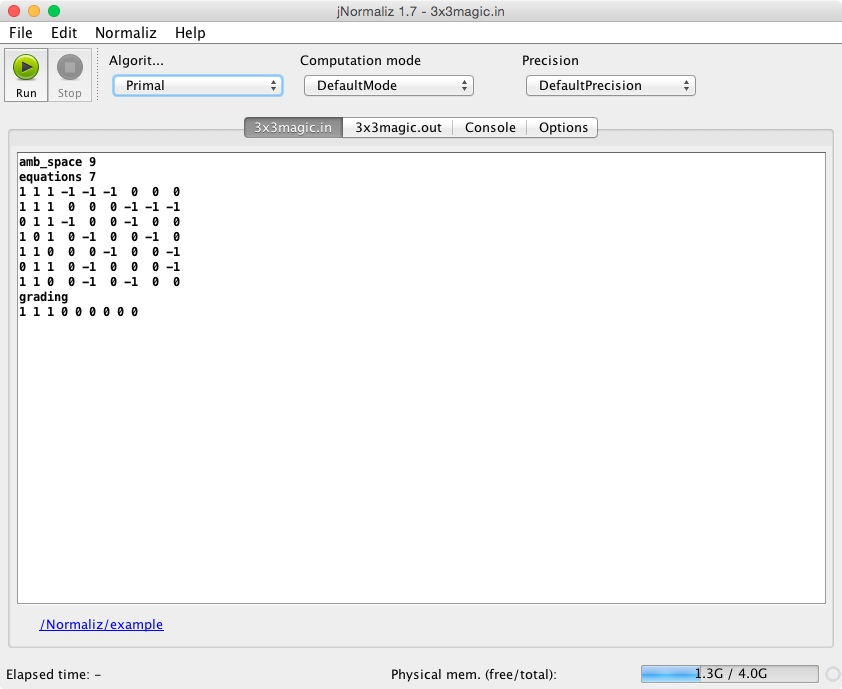
\includegraphics[width = 80 mm, bb=0 0 690 560]{jNormaliz.jpg}\\%width = 80 mm, bb=0 0 689 430
	\caption{jNormaliz}\label{new}
\end{figure}
In the jNormaliz file dialogue choose one of the input files
in the subdirectory \ttt{example}, say \ttt{small.in}, and
press \ttt{Run}. In the console window you can watch Normaliz
at work. Finally inspect the output window for the results.

The menus and dialogues of jNormaliz are self explanatory, but you
can also consult the documentation~\cite{AI} via the help menu.

\emph{Remark}\enspace The jNormaliz drop down menus do presently not cover all options of Normaliz. But since all computation goals and algorithmic variants can be set in the input file, there is no real restriction in using jNormaliz. The only option not reachable by jNormaliz is the output directory (see Section~\ref{outcontrol}).

Moreover, one can, and often will, run Normaliz from the
command line. This is fully explained in Section~\ref{options}. At this point it is enough to call Normaliz by typing
\begin{Verbatim}
normaliz -c <project>
\end{Verbatim}
where \ttt{<project>} denotes for the project to be computed. Normaliz will load the file \ttt{<project>.in}. The option \verb|-c| makes Normaliz to write a progress report on the terminal. Normaliz writes its results to \verb|<project>.out|.

Note that you may have to prefix \ttt{normaliz} by a path name, and \ttt{<project>} must contain a path to the input file if it is not in the current directory. Suppose the Normaliz directory is the current directory and we are using a Linux or Mac system. Then
\begin{Verbatim}
./normaliz -c example/small
\end{Verbatim}
will run \ttt{small.in} from the directory \ttt{example}. On Windows we must change this to
\begin{Verbatim}
.\normaliz -c example\small
\end{Verbatim}

The commands given above will run Normaliz with the at most $8$ parallel threads. For the very small examples in this tutorial you may want to add \ttt{-x=1} to suppress parallelization. For large examples, you can increase the number of parallel threads by \verb|-x=<N>| where \verb|<N>| is the number of threads that you want to suggest. See Section~\ref{exec}.

As long as you don't specify a computation goal on the command line or in the input file, Normaliz will use the \emph{default computation goals}:
\begin{verbatim}
HilbertBasis
HilbertSeries
ClassGroup
\end{verbatim}
The computation of the Hilbert series requires the explicit or implicit definition of a grading. Normaliz does only complain that a computation goal cannot be reached if the goal has been set explicitly.
For example, if you say \verb|HilbertSeries| and there is no grading, an exception will be thrown and Normaliz terminates, but an output file with the already computed data will be written.

Note that the spacing in the output files may have changed over time and that not all these changes may have made their way into this manual.

Normaliz will always print the results that are obtained on the way to the computation goals and do not require extra effort.

Appendix~\ref{Console} helps you to read the console output that you have demanded by the option \verb|-c|.
\subsection{A cone in dimension~$2$}\label{cone_ex}

We want to investigate the cone $C=\RR_+(2,1)+\RR_+(1,3)\subset \RR^2$:
\begin{center}
	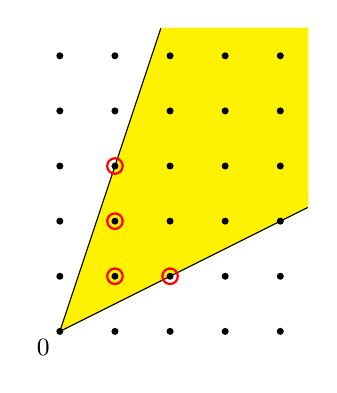
\begin{tikzpicture}[scale=0.7]
	\filldraw[yellow] (0,0) -- (1.833,5.5) -- (4.5,5.5) -- (4.5,2.25) -- cycle;
	\draw (0,0) -- (1.833,5.5);
	\draw (0,0) -- (4.5,2.25) node at (-0.3,-0.3){\small $0$};
	\foreach \x in {0,...,4}
	\foreach \y in {0,...,5}
	{
		\filldraw[fill=black] (\x,\y) circle (1.5pt);
	}
	\draw[red,thick] (1,1) circle (4pt);
	\draw[red,thick] (1,2) circle (4pt);
	\draw[red,thick] (1,3) circle (4pt);
	\draw[red,thick] (2,1) circle (4pt);
	\end{tikzpicture}
\end{center}

This cone is defined in the input file \verb|2cone.in|:
\begin{Verbatim}
amb_space 2
cone 2
1 3
2 1
\end{Verbatim}
The input tells Normaliz that the ambient space is $\RR^2$, and then a cone with~$2$ generators is defined, namely the cone $C$ from above.

The figure indicates the Hilbert basis, and this is our first computation goal.

If you prefer to consider the columns of a matrix as input vectors (or have a matrix in this format from another system) you can use the input
\begin{Verbatim}
amb_space 2
cone transpose 2
1 2
3 1
\end{Verbatim}
Note that the number \verb|2| following \verb|transpose| is now the number of \emph{columns}. Later on we will also show the use of formatted matrices.

\subsubsection{The Hilbert basis}
In order to compute the Hilbert basis, we run Normaliz from jNormaliz or by
\begin{Verbatim}
./normaliz -c example/2cone
\end{Verbatim}
and inspect the output file:
\begin{Verbatim}
4 Hilbert basis elements
2 extreme rays
2 support hyperplanes
\end{Verbatim}
Self explanatory so far.
\begin{Verbatim}
embedding dimension = 2
rank = 2 (maximal)
external index = 1
internal index = 5
original monoid is not integrally closed  in chosen lattice
\end{Verbatim}
The embedding dimension is the dimension of the space in which the computation is done. The rank is the rank of the lattice $\EE$ (notation as in Section~\ref{Term}). In fact, in our example $\EE=\ZZ^2$, and therefore has rank $2$.

For subgroups $G\subset U\subset \ZZ^d$ we denote the order of the torsion subgroup of $U/G$ by the \emph{index} of $G$ in $U$. The \emph{external index} is the index of the lattice $\EE$ in $\ZZ^d$. In our case $\EE=\ZZ^d$, and therefore the external index is $1$. Note: the external index is $1$ exactly when $\EE$ is a direct summand of $\ZZ^d$.

For this example and many others the \emph{original monoid} is well defined: the generators of the cone used as input are contained in $\EE$. (This need not be the case if $\EE$ is a proper sublattice of $\ZZ^d$, and we let the original monoid be undefined in inhomogeneous computations.) Let $G$ be the subgroup generated by the original monoid. The \emph{internal index} is the index of $G$ in $\EE$.

The original monoid is \emph{integrally closed} if and only if the it contains the Hilbert basis, and this is evidently false for our example. We go on.

\begin{Verbatim}
size of triangulation   = 1
resulting sum of |det|s = 5
\end{Verbatim}
The primal algorithm of Normaliz relies on a (partial) triangulation. In our case the triangulation consists of a single simplicial cone, and (the absolute value of) its determinant is~$5$.
\begin{Verbatim}
No implicit grading found
\end{Verbatim}
If you do not define a grading explicitly, Normaliz tries to find one itself: the grading is defined if and only if there is a linear form $\gamma$ on $\EE$ under which all extreme rays of the efficient cone $\CC$ have value $1$, and if so, $\gamma$ is the implicit grading. Such does not exist in our case.

The last information before we come to the vector lists:
\begin{Verbatim}
rank of class group = 0
finite cyclic summands:
5: 1  
\end{Verbatim}
The class group of the monoid $M$ has rank $0$, in other words, it is finite. It has one finite cyclic summand of order $5$.

This is the first instance of a multiset of integers displayed as a sequence of pairs
\begin{quote}
	\verb|<n>: <m>|
\end{quote}
Such an entry says: the multiset contains the number \verb|<n>| with multiplicity \verb|<m>.|


Now we look at the vector lists (typeset in two columns to save space):
\begin{Verbatim}
4 Hilbert basis elements:       2 extreme rays:
1 1                             1 3
1 2                             2 1
1 3
2 1                             2 support hyperplanes:
                                -1  2
                                 3 -1
\end{Verbatim}

The support hyperplanes are given by the linear forms (or inner normal vectors):
\begin{align*}
-x_1+2x_2&\ge 0,\\
3x_1-x_2&\ge 0.
\end{align*}

If the order is not fixed for some reason, Normaliz sorts vector lists as follows: (1) by degree if a grading exists and the application makes sense, (2) lexicographically.


\subsubsection{The cone by inequalities}\label{ineq_ex}

Instead by generators, we can define the cone by the inequalities just computed (\verb|2cone_ineq.in|). We use this example to show the input of a formatted matrix:
\begin{Verbatim}
amb_space auto
inequalities
[[-1  2] [3 -1]]
\end{Verbatim}
A matrix of input type \verb|inequalities| contains \emph{homogeneous} inequalities. Normaliz can determine the dimension of the ambient space from the formatted matrix. Therefore we can declare the ambient space as being ``auto determined'' (but \verb|amb_space 2| is not forbidden).

We get the same result as with \verb|2cone.in| except that the data depending on the original monoid cannot be computed: the internal index and the information on the original monoid are missing since there is no original monoid.

\subsubsection{The interior}\label{strict_ex}
Now we want to compute the lattice points in the interior of our cone. If the cone $C$ is given by the inequalities $\lambda_i(x)\ge0$ (within $\aff(C)$), then the interior is given by the inequalities $\lambda_i(x)>0$. Since we are interested in lattice points, we work with the inequalities $\lambda_i(x)\ge 1$.


The input file \verb|2cone_int.in| says
\begin{Verbatim}
amb_space 2
strict_inequalities 2
-1  2
3 -1
\end{Verbatim}
The strict inequalities encode the conditions
\begin{align*}
-x_1+2x_2&\ge 1,\\
3x_1-x_2&\ge 1.
\end{align*}
This is our first example of inhomogeneous input.

Note that the strict inequalities do not define the interior of the cone as a point set. They define a (closed) polyhedron with the same lattice points as the interior.

\begin{center}
	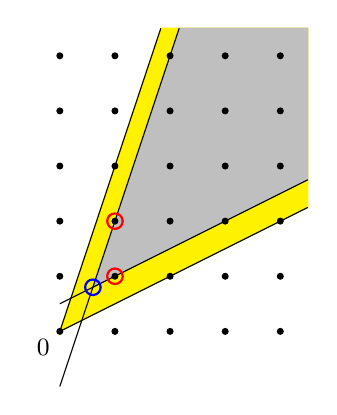
\begin{tikzpicture}[scale=0.7]
	\filldraw[yellow] (0,0) -- (1.833,5.5) -- (4.5,5.5) -- (4.5,2.25) -- cycle;
	\filldraw[lightgray] (0.6,0.8) -- (2.166,5.5) --(4.5,5.5) -- (4.5,2.75) -- cycle;
	\draw (0,0) -- (1.833,5.5);
	\draw (0,0) -- (4.5,2.25) node at (-0.3,-0.3){\small $0$};
	\draw (0,-1) -- (2.166,5.5);
	\draw (0,0.5) -- (4.5,2.75);
	\foreach \x in {0,...,4}
	\foreach \y in {0,...,5}
	{
		\filldraw[fill=black] (\x,\y) circle (1.5pt);
	}
	\draw[red,thick] (1,1) circle (4pt);
	\draw[red,thick] (1,2) circle (4pt);
	\draw[blue,thick] (0.6,0.8) circle (4pt);
	\end{tikzpicture}
\end{center}
Alternatively we could use the following two equivalent input files, in a more intuitive notation:
\begin{Verbatim}
amb_space 2
constraints 2
-1  2 > 0
3 -1 > 0
\end{Verbatim}
\begin{Verbatim}
amb_space 2
constraints 2
-1  2 >= 1
3 -1 >= 1
\end{Verbatim}
There is an even more intuitive way to type the input file using symbolic constraints that we will introduce in Section~\ref{cong_ex}.

Normaliz homogenizes inhomogeneous computations by introducing an auxiliary homogenizing coordinate $x_{d+1}$. The polyhedron is obtained by intersecting the homogenized cone with the hyperplane $x_{d+1}=1$. The recession cone is the intersection with the hyperplane $x_{d+1}=0$. The recession monoid is the monoid of lattice points in the recession cone, and the set of lattice points in the polyhedron is represented by its system of module generators over the recession monoid.

Note that the homogenizing coordinate serves as the denominator for rational vectors. In our example the recession cone is our old friend that we have already computed, and therefore we need not comment on it.

\begin{Verbatim}
2 module generators
4 Hilbert basis elements of recession monoid
1 vertices of polyhedron
2 extreme rays of recession cone
3 support hyperplanes of polyhedron (homogenized)

embedding dimension = 3
affine dimension of the polyhedron = 2 (maximal)
rank of recession monoid = 2
\end{Verbatim}
The only surprise may be the embedding dimension: Normaliz always takes the dimension of the space in which the computation is done. It is the number of components of the output vectors. Because of the homogenization it has increased by $1$.
\begin{Verbatim}
size of triangulation   = 1
resulting sum of |det|s = 25
\end{Verbatim}
In this case the homogenized cone has stayed simplicial, but the determinant has changed.
\begin{Verbatim}
dehomogenization:
0 0 1
\end{Verbatim}
The dehomogenization is the linear form $\delta$ on the homogenized space that defines the hyperplanes from which we get the polyhedron and the recession cone by the equations $\delta(x)=1$ and $\delta(x)=0$, respectively. It is listed since one can also work with a user defined dehomogenization.
\begin{Verbatim}
module rank = 1
\end{Verbatim}
This is the rank of the module of lattice points in the polyhedron over the recession monoid. In our case the module is an ideal, and so the rank is $1$.

The output of inhomogeneous computations is always given in homogenized form. The last coordinate is the value of the dehomogenization on the listed vectors, $1$ on the module generators, $0$ on the vectors in the recession monoid:
\begin{Verbatim}
2 module generators:          4 Hilbert basis elements of recession monoid:
1 1 1                         1 1 0
1 2 1                         1 2 0
                              1 3 0
                              2 1 0
\end{Verbatim}
The module generators are $(1,1)$ and $(1,2)$.
\begin{Verbatim}
1 vertices of polyhedron:
3 4 5
\end{Verbatim}
Indeed, the polyhedron has a single vertex, namely $(3/5,4/5)$.
\begin{Verbatim}
2 extreme rays of recession cone:     3 support hyperplanes of polyhedron (homogenized):
1 3 0                                 -1  2 -1
2 1 0                                  0  0  1
                                       3 -1 -1
\end{Verbatim}
Two support hyperplanes are exactly those that we have used to define the polyhedron -- and it has only $2$. But Normaliz always outputs the support hyperplanes that are needed for the cone that one obtains by homogenizing the polyhedron, as indicated by ``homogenized''. The homogenizing variable is always $\ge 0$. In this case the support hyperplane $(0,0,1)$ is essential for the description of the cone. Note that it need not always appear.


\subsection{A lattice polytope}\label{lattice_polytope}\label{polytope_ex}

\begin{minipage}[b]{0.5\textwidth}
	The file \ttt{polytope.in} contains
	
\begin{Verbatim}
amb_space 4
polytope 4
0 0 0
2 0 0
0 3 0
0 0 5
\end{Verbatim}
\end{minipage}
\hspace{1cm}
\begin{minipage}[t]{0.4\textwidth}
	\tikzset{facet style/.style={opacity=1.0,very thick,line,join=round}}
	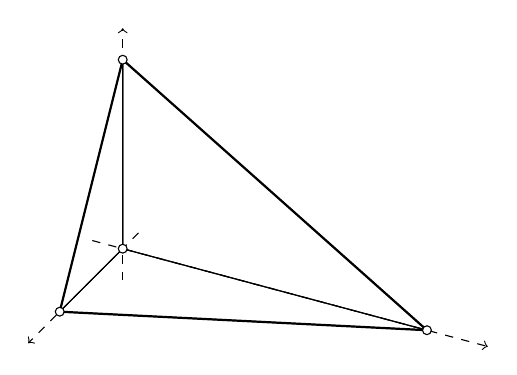
\begin{tikzpicture}[x = {(-0.5cm,-0.5cm)},
	y = {(0.9659cm,-0.25882cm)},
	z = {(0cm,1cm)},
	scale = 0.8]
	\draw [->,dashed] (-0.5, 0, 0) -- (3.0,0,0);
	
	\draw [->,dashed] (0, -0.5, 0) -- (0,6.0,0);
	
	\draw [->,dashed] (0, 0, -0.5) -- (0,0,3.5);
	
	\draw[thin] (0,0,0) -- (2,0,0) -- (0,5,0) -- cycle;
	\draw[thin] (0,0,0) -- (2,0,0) -- (0,0,3) -- cycle;
	\draw[thin] (0,0,0) -- (0,5,0) -- (0,0,3) -- cycle;
	\draw[thick] (2,0,0) -- (0,5,0) -- (0,0,3) -- cycle;
	
	\filldraw[fill=white] (0,0,0) circle (2pt);
	\filldraw[fill=white] (2,0,0) circle (2pt);
	\filldraw[fill=white] (0,5,0) circle (2pt);
	\filldraw[fill=white] (0,0,3) circle (2pt);
	\end{tikzpicture}
\end{minipage}

This is a good place to mention that Normaliz also accepts matrices (and vectors) in sparse format:

\begin{Verbatim}
amb_space 4
polytope 4 sparse
;
1:2;
2:3;
3:5;
\end{Verbatim}
Each input row, concluded by \verb|;|, lists the indices and the corresponding nonzero values in that row of the matrix.

The Ehrhart monoid of the integral polytope with the $4$
vertices
$$
(0,0,0)\,,\quad (2,0,0)\,,\quad (0,3,0)\quad\text{ and }\quad (0,0,5)
$$
in $\RR^3$ is to be computed. The generators of the Ehrhart monoid are obtained by attaching a further coordinate $1$ to the vertices, and this explains \verb|amb_space 4|. In fact, the input type \verb|polytope| is not only a convenient version of
\begin{Verbatim}
cone 4
0 0 0 1
2 0 0 1
0 3 0 1
0 0 5 1
\end{Verbatim}
It also sets the he grading to be the last coordinate. See~\ref{grading} below for general information on gradings.

Running \ttt{normaliz} produces the file \ttt{polytope.out}:
\begin{Verbatim}
19 Hilbert basis elements
18 lattice points in polytope (Hilbert basis elements of degree 1)
4 extreme rays
4 support hyperplanes

embedding dimension = 4
rank = 4 (maximal)
external index = 1
internal index = 30
original monoid is not integrally closed in chosen lattice
\end{Verbatim}
Perhaps a surprise: the lattice points of the polytope do not yield all Hilbert basis elements.
\begin{Verbatim}
size of triangulation   = 1
resulting sum of |det|s = 30
\end{Verbatim}
Nothing really new so far. The grading appears in the output file:
\begin{Verbatim}
grading:
0 0 0 1 

degrees of extreme rays:
1: 4
\end{Verbatim}
Again we encounter the notation \verb|<n>: <m>|: we have $4$ extreme rays, all of degree $1$.
\begin{Verbatim}
Hilbert basis elements are not of degree 1
\end{Verbatim}
We knew this already: the polytope is not integrally closed as defined in~\cite{BG}. Now we see the enumerative data defined by the grading:
\begin{Verbatim}
multiplicity = 30

Hilbert series:
1 14 15 
denominator with 4 factors:
1: 4  

degree of Hilbert Series as rational function = -2

Hilbert polynomial:
1 4 8 5 
with common denominator = 1
\end{Verbatim}
The polytope has $\ZZ^3$-normalized volume $30$ as indicated by the multiplicity (see Section~\ref{volume} for a discussion of volumes and multiplicities). The Hilbert (or Ehrhart) function counts the lattice points in $kP$, $k\in\ZZ_+$. The corresponding generating function is a
rational function $H(t)$. For our polytope it is
$$
\frac{1+14t+15t^2}{(1-t)^4}.
$$
The denominator is given in multiset notation: \verb|1: 4| say that the factor $(1-t^1)$ occurs with multiplicity $4$.

The Ehrhart polynomial (again we use a more general term in
the output file) of the polytope is
$$
p(k)=1+4k+8k^2+5k^3\,.
$$
In our case it has integral coefficients, a rare exception. Therefore one usually needs a denominator.

Everything that follows has already been explained.
\begin{Verbatim}
rank of class group = 0
finite cyclic summands:
30: 1  

***********************************************************************

18 lattice points in polytope (Hilbert basis elements of degree 1):
0 0 0 1
...
2 0 0 1

1 further Hilbert basis elements of higher degree:
1 2 4 2

4 extreme rays:                 4 support hyperplanes:
0 0 0 1                         -15 -10 -6 30
0 0 5 1                         0   0  1  0
0 3 0 1                         0   1  0  0
2 0 0 1                         1   0  0  0
\end{Verbatim}

The support hyperplanes give us a description of the polytope
by inequalities: it is the solution of the system of the $4$
inequalities
$$ x_3\ge0\,,\quad
x_2\ge0\,,\quad x_1\ge0\quad\text{ and }\quad
15x_1+10x_2+6x_3\le30\,.
$$

\subsubsection{Only the lattice points}\label{only_lattpoints}

Suppose we want to compute only the lattice points in our polytope. In the language of graded monoids these are the degree $1$ elements, and so we add \verb|Deg1Elements| to our input file (\verb|polytope_deg1.in|):
\begin{Verbatim}
amb_space 4
polytope 4
0 0 0
2 0 0
0 3 0
0 0 5
Deg1Elements
/* This is our first explicit computation goal*/
\end{Verbatim}
We have used this opportunity to include a comment in the input file. The computation of lattice points in a polytope will be taken up again in Sections~\ref{project_example} and~\ref{LattPoints}.

We lose all information on the Hilbert series, and from the Hilbert basis we only retain the degree $1$ elements.

\subsection{A rational polytope}\label{rational}

The type \verb|polytope| can (now) be used for rational polytopes as well.
\begin{center}
	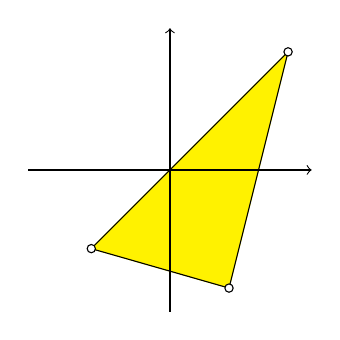
\begin{tikzpicture}[scale=3.0]
	\filldraw[yellow] (0.5,0.5) -- (-0.333,-0.333) -- (0.25,-0.5) -- cycle;
	\draw (0.5,0.5) -- (-0.333,-0.333) -- (0.25,-0.5) -- cycle;
	\draw[->] (0,-0.6) -- (0,0.6);
	\draw[->] (-0.6,0) -- (0.6,0);
	\filldraw[fill=white] (0.5,0.5) circle (0.5pt);
	\filldraw[fill=white] (-0.333,-0.333) circle (0.5pt);
	\filldraw[fill=white] (0.25,-0.5) circle (0.5pt);
	\end{tikzpicture}
\end{center}

We want to investigate the Ehrhart series of the triangle $P$
with vertices
$$
(1/2,1/2),\ (-1/3,-1/3),\ (1/4,-1/2).
$$
For this example the procedure above yields the input file \ttt{rational.in}:

\begin{Verbatim}
amb_space 3
polytope 3
1/2 1/2
-1/3 -1/3
1/4 -1/2
HilbertSeries
\end{Verbatim}

From the output file we only list the data of the Ehrhart series.
\begin{Verbatim}
multiplicity = 5/8
multiplicity (float) = 0.625

Hilbert series:
1 0 0 3 2 -1 2 2 1 1 1 1 2 
denominator with 3 factors:
1: 1  2: 1  12: 1  

degree of Hilbert Series as rational function = -3

Hilbert series with cyclotomic denominator:
-1 -1 -1 -3 -4 -3 -2 
cyclotomic denominator:
1: 3  2: 2  3: 1  4: 1  

Hilbert quasi-polynomial of period 12:
0:   48 28 15			7:   23 22 15
1:   11 22 15			8:   16 28 15
2:  -20 28 15			9:   27 22 15
3:   39 22 15			10:   -4 28 15
4:   32 28 15			11:    7 22 15
5:   -5 22 15			with common denominator = 48
6:   12 28 15
\end{Verbatim}
The multiplicity is a rational number. Since in dimension $2$
the normalized area (of full-dimensional polytopes) is twice
the Euclidean area, we see that $P$ has Euclidean area $5/16$. If the multiplicity is not integral, we also print it in floating point format, This is certainly superfluous for a fraction like $5/8$, but very handy if the numerator and the denominator have many digits.

Unlike in the case of a lattice polytope, there is no canonical choice of the denominator of the Ehrhart series. Normaliz gives it in $2$ forms. In the first form the numerator polynomial is
$$
1+3t^3+2t^4-t^5+2t^6+2t^7+t^8+t^9+t^{10}+t^{11}+2t^{12}
$$
and the denominator is
$$
(1-t)(1-t^2)(1-t^{12}).
$$
As a rational function, $H(t)$ has degree $-3$. This implies
that $3P$ is the smallest integral multiple of $P$ that
contains a lattice point in its interior.

Normaliz gives also a representation as a quotient of coprime
polynomials with the denominator factored into cyclotomic
polynomials. In this case
we have
$$
H(t)=-\frac{1+t+t^2+t^3+4t^4+3t^5+2t^6}{\zeta_1^3\zeta_2^2\zeta_3\zeta_4}
$$
where $\zeta_i$ is the $i$-th cyclotomic polynomial
($\zeta_1=t-1$, $\zeta_2=t+1$, $\zeta_3=t^2+t+1$,
$\zeta_4=t^2+1$).

Normaliz transforms the representation with cyclotomic
denominator into one with denominator of type
$(1-t^{e_1})\cdots(1-t^{e_r})$, $r=\textup{rank}$, by choosing
$e_r$ as the least common multiple of all the orders of the
cyclotomic polynomials appearing, $e_{r-1}$ as the lcm of those
orders that have multiplicity $\ge 2$ etc.

There are other ways to form a suitable denominator with $3$
factors $1-t^e$, for example
$g(t)=(1-t^2)(1-t^3)(1-t^4)=-\zeta_1^3\zeta_2^2\zeta_3\zeta_4$.
Of course, $g(t)$ is the optimal choice in this case. However,
$P$ is a simplex, and in general such optimal choice may not
exist. We will explain the reason for our standardization
below.

Let $p(k)$ be the number of lattice points in $kP$. Then $p(k)$
is a quasipolynomial:
$$
p(k)=p_0(k)+p_1(k)k+\dots+p_{r-1}(k)k^{r-1},
$$
where the coefficients depend on $k$, but only to the extent
that they are periodic of a certain period $\pi\in\NN$. In our
case $\pi=12$ (the lcm of the orders of the cyclotomic
polynomials).

The table giving the quasipolynomial is to be read as follows:
The first column denotes the residue class $j$ modulo the
period and the corresponding line lists the coefficients
$p_i(j)$ in ascending order of $i$, multiplied by the common
denominator. So
$$
p(k)=1+\frac{7}{12}k+\frac{5}{16}k^2, \qquad k\equiv 0\pod{12},
$$
etc. The leading coefficient is the same for all residue
classes and equals the Euclidean volume (in this case).

Our choice of denominator for the Hilbert series is motivated
by the following fact: $e_i$ is the common period of the
coefficients $p_{r-i},\dots,p_{r-1}$. The user should prove
this fact or at least verify it by several examples.

Especially in the case of a simplex the representation of the Hilbert series shown so far may not be the expected one. In fact, there is a representation in which the exponents of $t$ in the denominator are the degrees of the integral extreme generators. So one would expect the denominator to be $(1-t^2)(1-t^3)(1-t^4)$ in our case. The generalization to the nonsimplicial case uses the degrees of a homogeneous system of parameters (see~\cite[p.~200]{BG}). Normaliz can compute such a denominator if the computation goal \verb|HSOP| is set (\verb|rationalHSOP.in|):
\begin{Verbatim}
Hilbert series (HSOP):
1 1 1 3 4 3 2 
denominator with 3 factors:
2: 1  3: 1  4: 1 
\end{Verbatim}

Note that the degrees of the elements in a homogeneous system of parameters are by no means unique and that there is no optimal choice in general. To find a suitable sequence of degrees Normaliz must compute the face lattice of the cone to some extent. Therefore be careful not to ask for \verb|HSOP| if the cone has many support hyperplanes.

\subsubsection{The series with \ttt{vertices}?}

It is tempting to define the polytope by the input type \verb|vertices|. This choice makes the computation inhomogeneous, a mode that is mainly meant for (potentially) unbounded polyhedra. But it can be used for polytopes as well, and with this input type you can compute all of the data that we have seen above. You must ask for the \verb|EhrhartSeries| instead of the \verb|HilbertSeries|. The file \verb|rational_inhom.in| is
\begin{Verbatim}
amb_space 2
vertices 3
1/2 1/2 1
-1/3 -1/3 1
1/4 -1/2 1
EhrhartSeries
\end{Verbatim}

Nevertheless, there is also use for \verb|HilbertSeries| in the inhomogeneous case. But then the grading must be defined on the affine space of the polytope (and not on the cone over the polytope). See Sections~\ref{Polytopes} and~\ref{count}.

\subsubsection{The rational polytope by inequalities}\label{rat_ineq}

We extract the support hyperplanes of our polytope from the output file and use them as input (\verb|poly_ineq.in|):
\begin{Verbatim}
amb_space 3
inequalities 3
-8  2 3
1 -1 0
2  7 3
grading
unit_vector 3
HilbertSeries
\end{Verbatim}
At this point we have to help Normaliz because it has no way to guess that we want to investigate the polytope defined by the inequalities and the choice $x_3=1$. This is achieved by the specification of the grading that maps every vector to its third coordinate.

This is the first time that we used the shortcut \verb|unit_vector <n>| which represents the $n$-th unit vector $e_n\in\RR^d$ and is only allowed for input types which require a single vector.

These data tell us that the polytope, as a subset of $\RR^2$, is defined by the inequalities
\begin{align*}
-8x_1+2x_2+3&\ge0,\\
x_1-x_2+0&\ge0,\\
2x_1+7x_2+3&\ge 0.
\end{align*}
These inequalities are inhomogeneous, but we are using the homogeneous input type \verb|inequalities| which amounts to introducing the grading variable $x_3$ as explained above.


The inequalities as written above look somewhat artificial. It is certainly more natural to write them in the form
\begin{align*}
8x_1-2x_2&\le 3,\\
x_1-x_2&\ge0,\\
2x_1+7x_2&\ge -3.
\end{align*}
and for the direct transformation into Normaliz input we have introduced the type \verb|hom_constraints|. The prefix \verb|hom| indicates that we want homogeneous inequalities whereas plain \verb|constraints| that we have already seen in Section~\ref{strict_ex} gives inhomogeneous inequalities. The file \verb|poly_hom_const.in| contains
\begin{Verbatim}
amb_space 3
hom_constraints 3
8 -2 <= 3
1 -1 >= 0
2 7  >= -3
grading
unit_vector 3
HilbertSeries
\end{Verbatim}

You can of course also switch to inhomogeneous input using \verb|inhom_inequalities| or \verb|constraints| in the same way as \verb|polytope| can be replaced by \verb|vertices|.

\subsection{Magic squares}\label{eq_ex}

Suppose that you are interested in the following type of ``square''
\begin{center}
	\begin{tabular}{|l|l|l|}
		\hline
		$x_1$ & $x_2$ & $x_3$\\
		\hline
		$x_4$ & $x_5$ & $x_6$\\
		\hline
		$x_7$ & $x_8$ & $x_9$\\
		\hline
	\end{tabular}
\end{center}
and the problem is to find nonnegative values for $x_1,\dots,x_9$
such that the~$3$ numbers in all rows, all columns, and both
diagonals sum to the same constant $\mathcal{M}$. Sometimes
such squares are called \emph{magic} and $\mathcal M$ is the
\emph{magic constant}. This leads to a linear system of
equations
\begin{align*}
& x_1+x_2+x_3=x_4+x_5+x_6;\\
& x_1+x_2+x_3=x_7+x_8+x_9;\\
& x_1+x_2+x_3=x_1+x_4+x_7;\\
& x_1+x_2+x_3=x_2+x_5+x_8;\\
& x_1+x_2+x_3=x_3+x_6+x_9;\\
& x_1+x_2+x_3=x_1+x_5+x_9;\\
& x_1+x_2+x_3=x_3+x_5+x_7.\\
\end{align*}
This system is encoded in the file
\ttt{3x3magic.in}:
\begin{Verbatim}
amb_space 9
equations 7
1 1 1 -1 -1 -1  0  0  0
1 1 1  0  0  0 -1 -1 -1
0 1 1 -1  0  0 -1  0  0
1 0 1  0 -1  0  0 -1  0
1 1 0  0  0 -1  0  0 -1
0 1 1  0 -1  0  0  0 -1
1 1 0  0 -1  0 -1  0  0
grading
sparse 1:1 2:1 3:1;
\end{Verbatim}

The input type \verb|equations| represents \emph{homogeneous} equations. The first equation reads
$$
x_1+x_2+x_3-x_4-x_5-x_6=0,
$$
and the other equations are to be interpreted analogously. The magic constant is a natural choice for the grading. It is given in sparse form, equivalent to the dense form
\begin{Verbatim}
grading
1 1 1 0 0 0 0 0 0
\end{Verbatim}

It seems that we have forgotten to define the cone. This may indeed be the case, but doesn't matter: if there is no input type that defines a cone, Normaliz chooses the positive orthant, and this is exactly what we want in this case.

The output file contains the following:

\begin{Verbatim}
5 Hilbert basis elements
5 lattice points in polytope (Hilbert basis elements of degree 1)
4 extreme rays
4 support hyperplanes

embedding dimension = 9
rank = 3
external index = 1

size of triangulation   = 2
resulting sum of |det|s = 4

grading:
1 1 1 0 0 0 0 0 0 
with denominator = 3
\end{Verbatim}
The input degree is the magic constant. However, as the
denominator $3$ shows, the magic constant is always divisible
by $3$, and therefore the effective degree is $\mathcal M/3$.
This degree is used for the multiplicity, the Hilbert series, and the
Hilbert basis elements of degree $1$, and other date depending on the degree.

By introducing the grading denominator, Normaliz has changed the grading defined by you,
and you may not like this. There is a way out: add the option \verb|NoGradingDenom|. We will discuss the consequences below.
\begin{Verbatim}
degrees of extreme rays:
1: 4  

Hilbert basis elements are of degree 1
\end{Verbatim}
This was not to be expected (and is no longer true for $4\times 4$ squares).
\begin{Verbatim}
multiplicity = 4

Hilbert series:
1 2 1 
denominator with 3 factors:
1: 3  

degree of Hilbert Series as rational function = -1

Hilbert polynomial:
1 2 2 
with common denominator = 1
\end{Verbatim}
The Hilbert series is
$$
\frac{1+2t+t^2}{(1-t)^3}.
$$
The Hilbert polynomial is
$$
P(k)=1+2k+2k^2,
$$
and after substituting $\mathcal M/3$ for $k$ we obtain the
number of magic squares of magic constant $\mathcal M$, provided $3$ divides $\mathcal M$. (If $3\nmid \mathcal M$, there is no magic square of magic constant $\mathcal M$.)
\begin{Verbatim}
rank of class group = 1
finite cyclic summands:
2: 2  
\end{Verbatim}
So the class group is $\ZZ\oplus (\ZZ/2\ZZ)^2$.
\begin{Verbatim}
5 lattice points in polytope (Hilbert basis elements of degree 1):
0 2 1 2 1 0 1 0 2
1 0 2 2 1 0 0 2 1
1 1 1 1 1 1 1 1 1
1 2 0 0 1 2 2 0 1
2 0 1 0 1 2 1 2 0

0 further Hilbert basis elements of higher degree:
\end{Verbatim}
The $5$ elements of the Hilbert basis represent the magic
squares
\begin{center}
	\begin{tabular}{|l|l|l|}
		\hline
		2 & 0 & 1\\
		\hline
		0 & 1 & 2\\
		\hline
		1 & 2 & 0\\
		\hline
	\end{tabular}
	\hspace{10mm}
	\begin{tabular}{|l|l|l|}
		\hline
		1 & 0 & 2\\
		\hline
		2 & 1 & 0\\
		\hline
		0 & 2 & 1\\
		\hline
	\end{tabular}
	\hspace{10mm}
	\begin{tabular}{|l|l|l|}
		\hline
		1 & 1 & 1\\
		\hline
		1 & 1 & 1\\
		\hline
		1 & 1 & 1\\
		\hline
	\end{tabular}
	\hspace{10mm}
	\begin{tabular}{|l|l|l|}
		\hline
		1 & 2 & 0\\
		\hline
		0 & 1 & 2\\
		\hline
		2 & 0 & 1\\
		\hline
	\end{tabular}
	\hspace{10mm}
	\begin{tabular}{|l|l|l|}
		\hline
		0 & 2 & 1\\
		\hline
		2 & 1 & 0\\
		\hline
		1 & 0 & 2\\
		\hline
	\end{tabular}
\end{center}
All other solutions are linear combinations of these squares
with nonnegative integer coefficients.
One of these $5$ squares is clearly in the interior:
\begin{Verbatim}
4 extreme rays:                  4 support hyperplanes:
0 2 1 2 1 0 1 0 2                -2 -1 0 0  4 0 0 0 0
1 0 2 2 1 0 0 2 1                0 -1 0 0  2 0 0 0 0
1 2 0 0 1 2 2 0 1                0  1 0 0  0 0 0 0 0
2 0 1 0 1 2 1 2 0                2  1 0 0 -2 0 0 0 0
\end{Verbatim}

These $4$ support hyperplanes cut out the cone generated by the magic squares from the linear subspace they generate. Only one is reproduced as a sign inequality. This is due to the fact that the linear subspace has submaximal dimension and there is no unique lifting of linear forms to the full space.
\begin{Verbatim}
6 equations:                 3 basis elements of generated lattice:
1 0 0 0 0  1 -2 -1  1        1 0 -1 -2 0  2  1  0 -1
0 1 0 0 0  1 -2  0  0        0 1 -1 -1 0  1  1 -1  0
0 0 1 0 0  1 -1 -1  0        0 0  3  4 1 -2 -1  2  2
0 0 0 1 0 -1  2  0 -2
0 0 0 0 1 -1  1  0 -1
0 0 0 0 0  3 -4 -1  2
\end{Verbatim}
So one of our equations has turned out to be superfluous (why?). Note that also the equations are not reproduced exactly. Finally, Normaliz lists a basis of the efficient lattice $\EE$ generated by the magic squares.

Note that the equations and the lattice basis are not uniquely determined. We transform their matrices into reduced row echelon form to force unique output files.

\subsubsection{Blocking the grading denominator}\label{NoGradingDenominator}

As mentioned above, one can block the grading denominator and force Normaliz to use the input grading. For the magic squares we augment the input file as follows (\verb|3x3magicNGD.in|):
\begin{Verbatim}
amb_space 9
equations 7
1 1 1 -1 -1 -1  0  0  0
...
1 1 0  0 -1  0 -1  0  0
grading
sparse 1:1 2:1 3:1;
NoGradingDenom
\end{Verbatim}
The consequences:
\begin{Verbatim}
grading:
1 1 1 0 0 0 0 0 0 

degrees of extreme rays:
3: 4  

multiplicity = 4/9
multiplicity (float) = 0.444444444444

Hilbert series:
1 0 0 2 0 0 1 
denominator with 3 factors:
3: 3  

degree of Hilbert Series as rational function = -3

The numerator of the Hilbert series is symmetric.

Hilbert series with cyclotomic denominator:
-1 0 0 -2 0 0 -1 
cyclotomic denominator:
1: 3  3: 3  

Hilbert quasi-polynomial of period 3:
0:  9 6 2
1:  0 0 0
2:  0 0 0
with common denominator = 9

rank of class group = 1
finite cyclic summands:
2: 2  

***********************************************************************

0 lattice points in polytope (Hilbert basis elements of degree 1):
\end{Verbatim}

It is easy to relate the data with the grading denominator to those without. You must decide yourself what you prefer. One aspect is whether one prefers intrinsic data (with grading denominator) to extrinsic ones that depend on the embedding (without the grading denominator). We will discuss the topic again in Section~\ref{Polytopes}.

\subsubsection{With even corners}\label{magiceven}\label{cong_ex}

We change our definition of magic square by requiring that the
entries in the $4$ corners are all even. Then we have to
augment the input file by the following (\ttt{3x3magiceven.in}):
\begin{Verbatim}
congruences 4 sparse
1:1 10:2;
3:1 10:2;
7:1 10:2;
9:1 10:2;
\end{Verbatim}
This sparse form is equivalent to the dense form
\begin{Verbatim}
congruences 4
1 0 0 0 0 0 0 0 0 2
0 0 1 0 0 0 0 0 0 2
0 0 0 0 0 0 1 0 0 2
0 0 0 0 0 0 0 0 1 2
\end{Verbatim}
The first $9$ entries in each row represent the coefficients of the coordinates in the homogeneous congruences, and the last is the modulus:
$$
x_1\equiv 0\mod 2
$$
is the first congruence etc.

We could also define these congruences as symbolic constraints:
\begin{Verbatim}
constraints 4 symbolic
x[1] ~ 0(2);
x[3] ~ 0(2);
x[7] ~ 0(2);
x[9] ~ 0(2);
\end{Verbatim}

The output changes accordingly:


\begin{Verbatim}
9 Hilbert basis elements
0 lattice points in polytope (Hilbert basis elements of degree 1)
4 extreme rays
4 support hyperplanes

embedding dimension = 9
rank = 3
external index = 4

size of triangulation   = 2
resulting sum of |det|s = 8

grading:
1 1 1 0 0 0 0 0 0 
with denominator = 3

degrees of extreme rays:
2: 4  

multiplicity = 1

Hilbert series:
1 -1 3 1 
denominator with 3 factors:
1: 1  2: 2  

degree of Hilbert Series as rational function = -2

Hilbert series with cyclotomic denominator:
-1 1 -3 -1 
cyclotomic denominator:
1: 3  2: 2  

Hilbert quasi-polynomial of period 2:
0:   2 2 1
1:  -1 0 1
with common denominator = 2
\end{Verbatim}
After the extensive discussion in Section~\ref{rational} it should be easy for you to write down the Hilbert series and the Hilbert quasipolynomial. (But keep in mind that the grading has a denominator.)
\begin{Verbatim}
rank of class group = 1
finite cyclic summands:
4: 2  

***********************************************************************

0 lattice points in polytope (Hilbert basis elements of degree 1):

9 further Hilbert basis elements of higher degree:
...

4 extreme rays:
0 4 2 4 2 0 2 0 4
2 0 4 4 2 0 0 4 2
2 4 0 0 2 4 4 0 2
4 0 2 0 2 4 2 4 0
\end{Verbatim}
We have listed the extreme rays since they have changed after the introduction of the congruences, although the cone has not changed. The reason is that Normaliz always chooses the extreme rays from the efficient lattice $\EE$.
\begin{Verbatim}
4 support hyperplanes:
...

6 equations:
...                              3 basis elements of generated lattice:
                                   1 0 -1 -2 0  2  1  0 -1
2 congruences:                     0 1 -1 -1 0  1  1 -1  0
1 0 0 0 0 0 0 0 0 2                0 0  3  4 1 -2 -1  2  2
0 1 0 0 1 0 0 0 0 2
\end{Verbatim}
The rank of the lattice has of course not changed, but after the introduction of the congruences the basis has changed.

\subsubsection{The lattice as input}\label{latt_ex}

It is possible to define the lattice by generators. We demonstrate this for the magic squares with even corners. The lattice has just been computed (\verb|3x3magiceven_lat.in|):

\begin{Verbatim}
amb_space 9
lattice 3
0  1 2 3 1 -1 0  1 2
2 -1 2 1 1  1 0  3 0
0  3 0 1 1  1 2 -1 2
grading
1 1 1 0 0 0 0 0 0
\end{Verbatim}
It produces the same output as the version starting from equations and congruences.

\verb|lattice| has a variant that takes the saturation of the sublattice generated by the input vectors (\verb|3x3magic_sat.in|):

\begin{Verbatim}
amb_space 9
saturation 3
0  1 2 3 1 -1 0  1 2
2 -1 2 1 1  1 0  3 0
0  3 0 1 1  1 2 -1 2
grading
1 1 1 0 0 0 0 0 0
\end{Verbatim}
Clearly, we remove the congruences by this choice and arrive at the output of \verb|3x3magic.in|.

\subsection{Decomposition in a numerical semigroup}\label{inhom_eq_ex}

Let $S=\langle 6,10,15\rangle$, the numerical semigroup generated by $6,10,15$. How can $97$ be written as a sum in the generators?\medskip

In other words: we want to find all nonnegative integral solutions to the equation
$$
6x_1+10x_2+15x_3=97.
$$

\begin{minipage}[b]{0.5\textwidth}
	Input (\verb|NumSemi.in|):
\begin{Verbatim}
amb_space 3
constraints 1 symbolic
6x[1] + 10x[2] + 15x[3] = 97;
\end{Verbatim}
\end{minipage}
\hspace{1cm}
\begin{minipage}[t]{0.4\textwidth}
	\tikzset{facet style/.style={opacity=1.0,very thick,line,join=round}}
	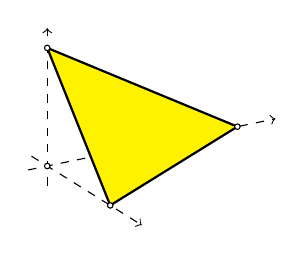
\begin{tikzpicture}[x = {(0.8cm,-0.5cm)},
	y = {(0.9659cm,0.20cm)},
	z = {(0cm,1cm)},
	scale = 0.5]
	\draw [->,dashed] (-0.5, 0, 0) -- (3.0,0,0);
	
	\draw [->,dashed] (0, -0.5, 0) -- (0,6.0,0);
	
	\draw [->,dashed] (0, 0, -0.5) -- (0,0,3.5);
	
	%\draw[thin] (0,0,0) -- (2,0,0) -- (0,5,0) -- cycle;
	%\draw[thin] (0,0,0) -- (2,0,0) -- (0,0,3) -- cycle;
	%\draw[thin] (0,0,0) -- (0,5,0) -- (0,0,3) -- cycle;
	\filldraw[color=yellow] (2,0,0) -- (0,5,0) -- (0,0,3) -- cycle;
	\draw[thick] (2,0,0) -- (0,5,0) -- (0,0,3) -- cycle;
	
	\filldraw[fill=white] (0,0,0) circle (2pt);
	\filldraw[fill=white] (2,0,0) circle (2pt);
	\filldraw[fill=white] (0,5,0) circle (2pt);
	\filldraw[fill=white] (0,0,3) circle (2pt);
	\end{tikzpicture}
\end{minipage}

\medskip
The equation cuts out a triangle from the positive orthant.

The set of solutions is a module over the monoid $M$ of solutions of the homogeneous equation $6x_1+10x_2+15x_3=0$. So $M=0$ in this case.
\begin{Verbatim}
6 lattice points in polytope (module generators):
2 1 5 1
2 4 3 1
2 7 1 1
7 1 3 1
7 4 1 1
12 1 1 1

0 Hilbert basis elements of recession monoid:
\end{Verbatim}
The last line is as expected, and the $6$ lattice points (or module generators) are the goal of the computation.

Normaliz is smart enough to recognize that it must compute the lattice points in a polygon, and does exactly this. You can recognize it in the console output: Normaliz \version\ has used the project-and-lift algorithm. We will discuss it further in Section~\ref{project_example} and Section~\ref{project}.

For those who like to play: add the option \verb|--NoProjection| to the command line. Then the terminal output will change; Normaliz computes the lattice points as a truncated Hilbert basis via a triangulation (only one simplicial cone in this case).

\subsection{A job for the dual algorithm}\label{job_dual}

We increase the size of the magic squares to $5\times 5$. Normaliz can do the same computation as for $3\times 3$ squares, but this will take some minutes. Suppose we are only interested in the Hilbert basis, we should use the dual algorithm for this example. (The dual algorithm goes back to Pottier~\cite{Po}.) The input file is \ttt{5x5dual.in}:

\begin{Verbatim}
amb_space 25
equations 11
1 1 1 1 1 -1 -1 -1 -1 -1  0  0  0  0  0  0  0  0  0  0  0  0  0  0  0
...
1 1 1 1 0  0  0  0 -1  0  0  0 -1  0  0  0 -1  0  0  0 -1  0  0  0  0
grading
1 1 1 1 1 0 0 0 0 0 0 0 0 0 0 0 0 0 0 0 0 0 0 0 0
HilbertBasis
\end{Verbatim}
The input file does not say anything about the dual algorithm mentioned in the section title. With this input it is chosen automatically. See Section~\ref{div_labor} for a discussion of when this happens. But you can insist on the dual algorithm by adding \verb|DualMode| to the input (or \verb|-d| to the command line). Or, if you want to compare it to the primal algorithm add \verb|PrimalMode| (or \verb|-P| to the command line).


The Hilbert basis contains $4828$ elements, too many to be listed here.

With the file \verb|5x5.in| you can compute the Hilbert basis and the Hilbert series, and the latter with HSOP:
\begin{Verbatim}
Hilbert series (HSOP):
1 15 356 4692 36324 198467 ... 198467 36324 4692 356 15 1 
denominator with 15 factors:
1: 5  2: 3  6: 2  12: 1  60: 2  420: 1  1260: 1  

degree of Hilbert Series as rational function = -5

The numerator of the Hilbert Series is symmetric.
\end{Verbatim}
In view of the length of the numerator of the Hilbert series it may be difficult to observe the symmetry. So Normaliz does it for you. The symmetry shows that the monoid is Gorenstein, but if you are only interested in the Gorenstein property, there is a much faster way to check it (see Section~\ref{Gorenstein}).

The size $6\times 6$ is out of reach for the Hilbert series, but the Hilbert basis can be computed (in the automatically chosen dual mode). It takes some hours.

\subsection{A dull polyhedron}\label{inhom_ineq_ex}

We want to compute the polyhedron defined by the inequalities
\begin{align*}
\xi_2 &\ge -1/2,\\
\xi_2 &\le 3/2,\\
\xi_2 &\le \xi_1+3/2.
\end{align*}
They are contained in the input file \verb|InhomIneq.in|:
\begin{Verbatim}
amb_space 2
constraints 3
0 1 >= -1/2
0 1 <=  3/2
-1 1 <=  3/2
grading
unit_vector 1
FVector
\end{Verbatim}
The grading says that we want to count points by the first coordinate, namely along the green lines:
\begin{center}
	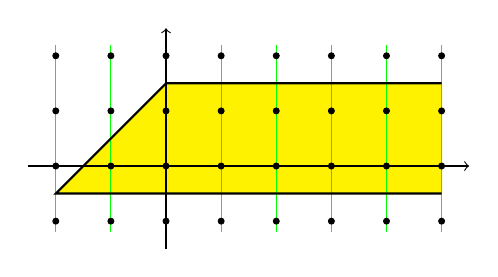
\begin{tikzpicture}[scale=0.7]
	
	\filldraw[yellow] (5,-0.5) -- (-2,-0.5) -- (0,1.5) -- (5,1.5) -- cycle;
	
	\foreach \x in {-2,...,5}
	{
		\draw[color=green] (\x,-1.2) -- (\x,2.2);
	}
	
	\foreach \x in {-2,...,5}
	\foreach \y in {-1,...,2}
	{
		\filldraw[fill=black] (\x,\y) circle (1.5pt);
	}
	\draw[->] (-2.5,0) -- (5.5,0);
	\draw[->] (0,-1.5) -- (0,2.5);
	\draw[thick] (5,-0.5) -- (-2,-0.5) -- (0,1.5) -- (5,1.5);
	
	\end{tikzpicture}
\end{center}

It yields the output
\begin{Verbatim}
2 module generators
1 Hilbert basis elements of recession monoid
2 vertices of polyhedron
1 extreme rays of recession cone
3 support hyperplanes of polyhedron (homogenized)

f-vector:
1 2 3 1 
\end{Verbatim}
The empty set is the intersection of all facets, and this gives the first entry $1$. Then we have $2$ vertices, $3$ edges, and finally the full polyhedron.

The out put continues:

\begin{Verbatim}
embedding dimension = 3
affine dimension of the polyhedron = 2 (maximal)
rank of recession monoid = 1

size of triangulation   = 1
resulting sum of |det|s = 8

dehomogenization:
0 0 1 

grading:
1 0 0 
\end{Verbatim}
The interpretation of the grading requires some care in the inhomogeneous case. We have extended the input grading vector by an entry $0$ to match the embedding dimension. For the computation of the degrees of \emph{lattice points} in the ambient space you can either use only the first $2$ coordinates or take the full scalar product of the point in homogenized coordinates and the extended grading vector.

\begin{Verbatim}
module rank = 2
multiplicity = 2
\end{Verbatim}
The module rank is $2$ in this case since we have two ``layers'' in the solution module that are parallel to the recession monoid. This is of course also reflected in the Hilbert series.
\begin{Verbatim}
Hilbert series:
1 1 
denominator with 1 factors:
1: 1  

shift = -1
\end{Verbatim}
We haven't seen a shift yet. It is always printed (necessarily) if the Hilbert series does not start in degree $0$. In our case it starts in degree $-1$ as indicated by the shift $-1$. We thus get the Hilbert series
$$
t^{-1}\,\frac{t+t}{1-t}=\frac{t^{-1}+1}{1-t}.
$$

Note: We used the opposite convention for the shift in Normaliz~2.

Note that the Hilbert (quasi)polynomial is always computed for the unshifted monoid defined by the input data. (This was different in previous versions of Normaliz.)
\begin{Verbatim}
degree of Hilbert Series as rational function = -1

Hilbert polynomial:
2 
with common denominator = 1

***********************************************************************

2 module generators:
-1 0 1
0 1 1

1 Hilbert basis elements of recession monoid:
1 0 0

2 vertices of polyhedron:
-4 -1 2
0  3 2

1 extreme rays of recession cone:
1 0 0

3 support hyperplanes of polyhedron (homogenized):
0 -2 3
0  2 1
2 -2 3
\end{Verbatim}

The dual algorithm that was used in Section~\ref{job_dual} can also be applied to inhomogeneous computations. We would of course loose the Hilbert series. In certain cases it may be preferable to suppress the computation of the vertices of the polyhedron if you are only interested in the integer points; see Section~\ref{InhomDual}.

\subsubsection{Defining it by generators}\label{polyh_ex}

If the polyhedron is given by its vertices and the recession cone, we can define it by these data (\verb|InhomIneq_gen.in|):
\begin{Verbatim}
amb_space 2
vertices 2
-4 -1 2
0  3 2
cone 1
1 0
grading
unit_vector 1
\end{Verbatim}
The output is identical to the version starting from the inequalities.

\subsection{The Condorcet paradox}\label{Condorcet}

In social choice elections each of the $k$ voters picks a linear preference order of the $n$ candidates. There are $n!$ such orders. The election result is the vector $(x_1,\dots,x_N)$, $N=n!$, in which $x_i$ is the number of voters that have chosen the $i$-th preference order in, say, lexicographic enumeration of these orders. (Thus $x_1+\dots+x_N=k$.) In the following we assume the \emph{impartial anonymous culture} according to which every election result has the same probability if the number of voters is fixed.
\medskip

We say that candidate $A$ \emph{beats} candidate $B$ if the majority of the voters prefers $A$ to $B$. As the Marquis de \emph{Condorcet} (and others) observed, ``beats'' is not transitive, and an election may exhibit the \emph{Condorcet paradox}: there is no Condorcet winner. (See~\cite{BS} and the references given there for more information.)

We want to find the probability for $k\to\infty$ that there is a Condorcet winner for $n=4$ candidates. The event that $A$ is the Condorcet winner can be expressed by linear inequalities on the election outcome (a point in $24$-space). The wanted probability is the lattice normalized volume of the polytope cut out by the inequalities at $k=1$. The file \verb|Condorcet.in|:

\begin{Verbatim}
amb_space 24
inequalities 3
1 1 1 1 1 1 -1 -1 -1 -1 -1 -1   1  1 -1 -1  1 -1   1  1 -1 -1  1 -1
1 1 1 1 1 1  1  1 -1 -1  1 -1  -1 -1 -1 -1 -1 -1   1  1  1 -1 -1 -1
1 1 1 1 1 1  1  1  1 -1 -1 -1   1  1  1 -1 -1 -1  -1 -1 -1 -1 -1 -1
nonnegative
total_degree
Multiplicity
\end{Verbatim}
The first inequality expresses that $A$ beats $B$, the second and the third say that $A$ beats $C$ and $D$. (So far we do not exclude ties, and they need not be excluded for probabilities as $k\to\infty$.)

In addition to these inequalities we must restrict all variables to nonnegative values, and this is achieved by adding the attribute \verb|nonnegative|. The grading is set by \verb|total_degree|. It replaces the grading vector with $24$ entries $1$. Finally \verb|Multiplicity| sets the computation goal.

From the output file we only mention the quantity we are out for:
\begin{Verbatim}
multiplicity = 1717/8192
multiplicity (float) = 0.209594726562
\end{Verbatim}
Since there are $4$ candidates, the probability for the existence of a Condorcet winner is $1717/2048=0.209595$.

We can refine the information on the Condorcet paradox by computing the Hilbert series. Either we delete \verb|Multiplicity| from the input file or, better, we add \verb|--HilbertSeries| (or simply \verb|-q|) on the command line. The result:
\begin{Verbatim}
Hilbert series:
1 5 133 363 4581 8655 69821 100915 ... 12346 890 481 15 6 
denominator with 24 factors:
1: 1  2: 14  4: 9

degree of Hilbert Series as rational function = -25
\end{Verbatim}

If your executable of Normaliz was built with CoCoALib (see Section~\ref{Compile}), for example the executables for Linux or Mac~OS from our distribution or in the Docker image, it uses symmetrization for the computation of the Hilbert series. If not, then simply disregard any remark on symmetrization. Everything runs very quickly also without it.

If symmetrization has been used, you will also find a file \verb|Condorcet.symm.out| in your directory. It contains the data computed for the symmetrization. You need not care at this point. We take continue the discussion of symmetrization in Section~\ref{symmetrize}.

\subsubsection{Excluding ties}\label{excluded_ex}

Now we are more ambitious and want to compute the Hilbert series for the Condorcet paradox, or more precisely, the number of election outcomes having $A$ as the Condorcet winner depending on the number $k$ of voters. Moreover, as it is customary in social choice theory, we want to exclude ties. The input file changes to \verb|CondorcetSemi.in|:
\begin{Verbatim}
amb_space 24
excluded_faces 3
1 1 1 1 1 1 -1 -1 -1 -1 -1 -1   1  1 -1 -1  1 -1   1  1 -1 -1  1 -1
1 1 1 1 1 1  1  1 -1 -1  1 -1  -1 -1 -1 -1 -1 -1   1  1  1 -1 -1 -1
1 1 1 1 1 1  1  1  1 -1 -1 -1   1  1  1 -1 -1 -1  -1 -1 -1 -1 -1 -1
nonnegative
total_degree
HilbertSeries
\end{Verbatim}
We could omit \verb|HilbertSeries|, and the computation would include the Hilbert basis. The type \verb|excluded_faces| only affects the Hilbert series. In every other respect it is equivalent to \verb|inequalities|.

From the file \verb|CondorcetSemi.out| we only display the Hilbert series:
\begin{Verbatim}
Hilbert series:
6 15 481 890 12346 ... 100915 69821 8655 4581 363 133 5 1 
denominator with 24 factors:
1: 1  2: 14  4: 9  

shift = 1

degree of Hilbert Series as rational function = -24
\end{Verbatim}
Surprisingly, this looks like the Hilbert series in the previous section read backwards, roughly speaking. This is true, and one can explain it as we will see below.

It is justified to ask why we don't use \verb|strict_inequalities| instead of \verb|excluded_faces|. It does of course give the same Hilbert series. However, Normaliz cannot (yet) apply symmetrization in inhomogeneous computations. Moreover, the algorithmic approach is different, and according to our experience \verb|excluded_faces| is more efficient, independently of symmetrization.

See Section~\ref{semi_open} for more information on \verb|excluded_faces|.

\subsubsection{At least one vote for every preference order}\label{strict_signs_ex}

Suppose we are only interested in elections in which every preference order is chosen by at least one voter. This can be modeled as follows (\verb|Condorcet_one.in|):
\begin{Verbatim}
amb_space 24
inequalities 3
1 1 1 1 1 1 -1 -1 -1 -1 -1 -1   1  1 -1 -1  1 -1   1  1 -1 -1  1 -1
1 1 1 1 1 1  1  1 -1 -1  1 -1  -1 -1 -1 -1 -1 -1   1  1  1 -1 -1 -1
1 1 1 1 1 1  1  1  1 -1 -1 -1   1  1  1 -1 -1 -1  -1 -1 -1 -1 -1 -1
strict_signs
1 1 1 1 1 1 1 1 1 1 1 1 1 1 1 1 1 1 1 1 1 1 1 1
total_degree
HilbertSeries
\end{Verbatim}
The entry $1$ at position $i$ of the vector \verb|strict_signs| imposes the inequality $x_i\ge1$. A $-1$ would impose the inequality $x_i\le -1$, and the entry $0$ imposes no condition on the $i$-th coordinate.

\begin{Verbatim}
Hilbert series:
1 5 133 363 4581 8655 69821 100915 ... 12346 890 481 15 6 
denominator with 24 factors:
1: 1  2: 14  4: 9  

shift = 24

degree of Hilbert Series as rational function = -1
\end{Verbatim}
Again we encounter (almost) the Hilbert series of the Condorcet paradox (without side conditions). It is time to explain this coincidence. Let $C$ be the Condorcet cone defined by the nonstrict inequalities, $M$ the monoid of lattice points in it, $I_1\subset M$ the ideal of lattice points avoiding the $3$ facets defined by ties, $I_2$ the ideal of lattice points with strictly positive coordinates, and finally $I_3$ the ideal of lattice points in the interior of $C$. Moreover, let $\mathds{1}\in\ZZ^{24}$ be the vector with all entries $1$.

Since $\mathds{1}$ lies in the three facets defining the ties, it follows that $I_2=M+\mathds{1}$. This explains why we obtain the Hilbert series of $I_2$ by multiplying the Hilbert series of $M$ by $t^{24}$, as just observed. Generalized Ehrhart reciprocity (see~\cite[Theorem~6.70]{BG}) then explains the Hilbert series of $I_1$ that we observed in the previous section. Finally, the Hilbert series of $I_3$ that we don't have displayed is obtained from that of $M$ by ``ordinary'' Ehrhart reciprocity. But we can also obtain $I_1$ from $I_3$: $I_1=I_3-\mathds{1}$, and generalized reciprocity follows from ordinary reciprocity in this very special case. (Also see~\cite{BIS2}.)

The essential point in these arguments (apart from reciprocity) is that $\mathds{1}$ lies in all support hyperplanes of $C$ except the coordinate hyperplanes.

You can easily compute the Hilbert series of $I_3$ by making all inequalities strict.

As the terminal output shows, symmetrization has not been applied for the reason mentioned above: \verb|strict_signs| is an inhomogeneous input type. It would of course be possible to encode the strict signs as \verb|excluded_faces|. Then the sparse format of matrices is very handy:
\begin{Verbatim}
excluded_faces 24
1:1;
1:2;
...
1:24;
\end{Verbatim}
This is a shorthand for the unit matrix.

\subsubsection{The f-vector with codimension bound}\label{codim_bound}

Suppose we are interested in the f-vector of the cone defined by \ttt{Condorcet.in}. In view of the rather high dimension the face lattice must be expected to be extremely large, but computing the f-vector to codimension $4$ should be no problem. (See~\cite{BGOW} for the Normaliz face lattice algorithm.) Indeed it is not. We use \ttt{CondorcetFV.in}:
\begin{Verbatim}
...
FVector
face_codim_bound 4
\end{Verbatim}

Then we find in the output file:
\begin{Verbatim}
f-vector (possibly truncated):
17550 2925 351 27 1
\end{Verbatim}
Note that the face numbers are listed by descending codimension or, equivalently, by increasing dimension. The leftmost number is the number of faces in the highest codimension that has been computed. So we have $17550$ codimension $4$ faces.


\subsection{Testing normality}\label{normalization_ex}

We want to test the monoid $A_{4\times 4\times 3}$ defined by $4\times4\times3$ contingency tables for normality (see~\cite{BHIKS} for the background). The input file is \ttt{A443.in}:
\begin{Verbatim}
amb_space 40
cone_and_lattice 48
1 0 0 0 0 0 0 0 0 0 0 0 0 0 0 0 1 0 0 0 0 0 0 0 0 0 0 0 1 0 0 0 0 0 0 0 0 0 0 0
...
0 0 0 0 0 0 0 0 0 0 0 0 0 0 0 1 0 0 0 0 0 0 0 0 0 0 0 1 0 0 0 0 0 0 0 0 0 0 0 1
HilbertBasis
\end{Verbatim}
Why \verb|cone_and_lattice|? Well, we want to find out whether the monoid is normal, i.e., whether $M=C(M)\cap\gp(M)$. If $M$ is even integrally closed in $\ZZ^{24}$, then it is certainly integrally closed in the evidently smaller lattice $\gp(M)$, but the converse does not hold in general, and therefore we work with the lattice generated by the monoid generators.

It turns out that the monoid is indeed normal:
\begin{Verbatim}
original monoid is integrally closed in chosen lattice
\end{Verbatim}
Actually the output file reveals that $M$ is even integrally closed in $\ZZ^{24}$: the external index is $1$, and therefore $\gp(M)$ is integrally closed in $\ZZ^{24} $.

The output file also shows that there is a grading on $\ZZ^{24}$ under which all our generators have degree $1$. We could have seen this ourselves: Every generator has exactly one entry $1$ in the first $16$ coordinates. (This is clear from the construction of $M$.)

A noteworthy detail from the output file:
\begin{Verbatim}
size of partial triangulation   = 48
\end{Verbatim}
It shows that Normaliz uses only a partial triangulation in Hilbert basis computations; see~\cite{BHIKS}.

It is no problem to compute the Hilbert series as well if you are interested in it. Simply add \verb|-q| to the command line or remove \verb|HilbertBasis| from the input file. Then a full triangulation is needed (size $2,654,272$).

Similar examples are \verb|A543|, \verb|A553| and \verb|A643|. The latter is not normal, as we will see below. Even on a standard PC or laptop, the Hilbert basis computation does not take very long because Normaliz uses only a partial triangulation. The Hilbert series can still be determined, but the computation time will grow considerably since the it requires a full triangulation. See~\cite{BIS} for timings.

\subsubsection{Computing just a witness}\label{IsIC}

If the Hilbert basis is large and there are many support hyperplanes, memory can become an issue for Normaliz, as well as computation time. Often one is only interested in deciding whether the given monoid is integrally closed (or normal). In the negative case it is enough to find a single element that is not in the original monoid -- a witness disproving integral closedness. As soon as such a witness is found, Normaliz stops the Hilbert basis computation (but will continue to compute other data if they are asked for). We look at the example \verb|A643.in| (for which the full Hilbert basis is not really a problem):


\begin{Verbatim}
amb_space 54
cone_and_lattice 72
1 0 0 0 0 0 0 0 0 0 0 0 0 0 0 0 0 0 0 0 0 0 0 0 1 0 ...
...
0 0 0 0 0 0 0 0 0 0 0 0 0 0 0 0 0 0 0 0 0 0 0 1 0 0 ...
WitnessNotIntegrallyClosed
\end{Verbatim}
Don't add \verb|HilbertBasis| because it will overrule \verb|IsIntegrallyClosed|!

The output:
\begin{Verbatim}
72 extreme rays
153858 support hyperplanes

embedding dimension = 54
rank = 42
external index = 1
internal index = 1
original monoid is not integrally closed in chosen lattice
witness for not being integrally closed:
0 0 1 0 1 1 1 1 0 0 1 0 0 1 0 1 0 1 1 0 1 1 0 0 1 1 1 0 0 1 1 0 0 1 1 ...

grading:
1 1 1 1 1 1 1 1 1 1 1 1 1 1 1 1 1 1 1 1 1 1 1 1 0 0 0 0 0 0 0 0 0 0 0 ...

degrees of extreme rays:
1: 72  

***********************************************************************

72 extreme rays:
0 0 0 0 0 0 0 0 0 0 0 0 0 0 0 0 0 0 0 0 0 0 0 1 0 0 0 0 0 0 0 0 0 0 0 0 ...
...
\end{Verbatim}

If you repeat such a computation, you may very well get a different witness if several parallel threads find witnesses. Only one of them is delivered.

If you just want to check integral closedness as quickly as possible, replace \verb|WitnessNotIntegrallyClosed| by \verb|IsIntegrallyClosed|. Normaliz first checks some necessary conditions. If they are satisfied, the calculation of the Hilbert basis is started. If it finds a witness for not being integrally closed, the witness is displayed in the output.
\subsection{Convex hull computation/vertex enumeration}

Normaliz computes convex hulls as should be very clear by now, and the only purpose of this section is to emphasize that Normaliz can be restricted to this task by setting an explicit computation goal. By convex hull computation we mean the determination of the support hyperplanes of a polyhedron is given by generators (or vertices). The converse operation is vertex enumeration. Both amount to the dualization of a cone, and can therefore be done by the same algorithm.

As an example we take the input file \verb|cyclicpolytope30-15.in|, the cyclic polytope of dimension~$15$ with~$30$ vertices (suggested by D.~Avis and Ch.~Jordan):
\begin{Verbatim}
/* cyclic polytope of dimension 15 with 30 vertices */
amb_space 16
polytope 30
1 1 1 1 1 1 1 1 1 1 1 1 1 1 1
2 4 8 16 32 64 128 256 512 1024 2048 4096 8192 16384 32768
...
30 900 27000 810000 ... 478296900000000000000 14348907000000000000000
SupportHyperplanes
\end{Verbatim}
Already the entries of the vertices show that the computation cannot be done in~$64$~bit arithmetic. But you need not be worried. Just start Normaliz as usual. It will simply switch to infinite precision by itself, as shown by the terminal output (use the option \verb|-c| or \verb|--Verbose|).
\begin{Verbatim}
\.....|
Normaliz 3.2.0                   \....|
\...|
(C) The Normaliz Team, University of Osnabrueck   \..|
January  2017                       \.|
\|
************************************************************
Compute: SupportHyperplanes
Could not convert 15181127029874798299.
Arithmetic Overflow detected, try a bigger integer type!
Restarting with a bigger type.
************************************************************
starting primal algorithm (only support hyperplanes) ...
Generators sorted lexicographically
Start simplex 1 2 3 4 5 6 7 8 9 10 11 12 13 14 15 16 
gen=17, 72 hyp
gen=18, 240 hyp
gen=19, 660 hyp
gen=20, 1584 hyp
gen=21, 3432 hyp
gen=22, 6864 hyp
gen=23, 12870 hyp
gen=24, 22880 hyp
gen=25, 38896 hyp
gen=26, 63648 hyp
gen=27, 100776 hyp
gen=28, 155040 hyp
gen=29, 232560 hyp
gen=30, 341088 hyp
Pointed since graded
Select extreme rays via comparison ... done.
------------------------------------------------------------
transforming data... done.
\end{Verbatim}
Have a look at the output file if you are not afraid of $341088$ linear forms.

If you have looked closely at the terminal output above, you should have stumbled on the lines
\begin{Verbatim}
Could not convert 15181127029874798299.
Arithmetic Overflow detected, try a bigger integer type!
\end{Verbatim}
They show that Normaliz has tried the computation in~$64$~bit integers, but encountered a number that is too large for this precision. It has automatically switched to infinite precision. (See Section~\ref{Integer} for more information on integer types.)

\subsection{Lattice points in a polytope and its Euclidean volume}\label{project_example}

The computation of lattice points in a polytope can be viewed as a truncated Hilbert basis computation, and we have seen in preceding examples. But Normaliz can be restricted to their computation, with homogeneous as well as with inhomogeneous input. Let us look at \verb|ChF_8_1024.in|:

\begin{Verbatim}
amb_space 8
constraints 16
0.10976576 0.2153132834 ... 0.04282847494 >= -1/2
...
0.10976576 -0.2153132834 ... -0.04282847494 >= -1/2
0.10976576 0.2153132834 ... 0.04282847494 <= 1/2
0.10976576 -0.2153132834 ...-0.04282847494 <= 1/2
LatticePoints
ProjectionFloat
\end{Verbatim}

This example comes from numerical analysis; see Ch.~Kacwin, J.~Oettershagen and T.~Ullrich, On the orthogonality of the Chebyshev-Frolov lattice and applications, Monatsh.\ Math.\ 184 (2017), 425--441). Its origin explains the decimal fractions in the input. Normaliz converts them immediately into ordinary fractions of type numerator/denominator, and then makes the input integral as usual.

In the output file you can see to what integer vectors Normaliz has converted the inequalities of the input file:
\begin{Verbatim}
16 support hyperplanes of polyhedron (homogenized):
5488288000  10765664170  ...  2141423747 25000000000
...
-5488288000  10765664170 ...   2141423747 25000000000
\end{Verbatim}

The option \verb|ProjectionFloat| indicates that we want to compute the lattice points in the polytope defined by the inequalities and that we want to use the floating point variant of the project-and-lift algorithm; \verb|Projection| would make Normaliz use its ordinary arithmetic in this algorithm. For our example the difference in time is not really significant, but when you try \verb|VdM_16_1048576.in|, it becomes very noticeable. Let us have a look at the relevant part of then terminal output:
\begin{Verbatim}
Polyhedron is parallelotope
Computing lattice points by project-and-lift
LLL based on support hyperplanes
Projection
embdim 9 inequalities 16
...
embdim 6 inequalities 140
...
embdim 2 inequalities 2
embdim 1 inequalities 0
Lifting
Lifting to dimension 2
Lifting to dimension 3
...
Lifting to dimension 8
Lifting to dimension 9
embdim 2 LatticePoints 5
embdim 3 LatticePoints 21
...
embdim 8 LatticePoints 907
embdim 9 LatticePoints 1067
Project-and-lift complete
\end{Verbatim}

We start with embedding dimension~$9$ since we need a homogenizing coordinate in inhomogeneous computations. Then the polytope is successively projected onto a coordinate hyperplane until we reach a line segment given by~$2$ inequalities. In the second part Normaliz lifts the lattice points back through all projections. The following figure illustrates the procedure for a polygon that is projected to a line segment.
\begin{center}
	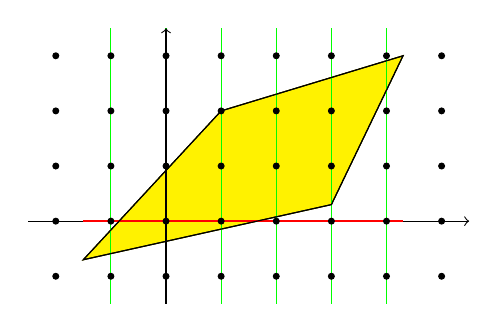
\begin{tikzpicture}[scale=0.7]
	
	\filldraw[yellow] (-1.5,-0.7) -- (1,2) -- (4.3,3) -- (3,0.3) -- cycle;
	\draw (-1.5,-0.7) -- (1,2) -- (4.3,3) -- (3,0.3) -- cycle;
	
	\foreach \x in {-1,...,4}
	{
		\draw[green] (\x,-1.5) -- (\x,3.5);
	}
	\draw[->] (-2.5,0) -- (5.5,0);
	\draw[->] (0,-1.5) -- (0,3.5);
	%\draw (-1.5,-1.5) -- (-1.5,3.5);
	\draw[color=red,thick] (-1.5,0) -- (4.3,0);
	
	\foreach \x in {-2,...,5}
	\foreach \y in {-1,...,3}
	{
		\filldraw[fill=black] (\x,\y) circle (1.5pt);
	}
	\draw (-1.5,-0.7) -- (1,2) -- (4.3,3) -- (3,0.3) -- cycle;
	%\draw[thick] (5,0) -- (-1,-0) -- (0,1) -- (5,1);
	\end{tikzpicture}
\end{center}
The green lines show the fibers over the lattice points in the (red) line segment. Note that not every lattice point in the projection must be liftable to a lattice point in the next higher dimension.

In \verb|ChF_8_1024.out| we see
\begin{Verbatim}
1067 lattice points in polytope (module generators):
-4  0  0  0  0  0  0  0 1
-3  0  0  0 -1  0  0  0 1
-3  0  0  0  0  0  0  0 1
...
3  0  0  0  0  0  0  0 1
3  0  0  0  1  0  0  0 1
4  0  0  0  0  0  0  0 1
\end{Verbatim}

Normaliz finds out that our polytope is in fact a parallelotope. This allows Normaliz to suppress the computation of its vertices. We are not interested in them, and they look frightening when written as ordinary fractions (computed with the additional option \verb|SupportHyperplanes|). This is only the first vertex, the denominator is the number in the last row:
\begin{Verbatim}
256 vertices of polyhedron:
-7831972155307708173239167258085974255845869779051329651906336771582421875
-2560494334732147696394408175864650673712115229853232268085759500000000000
2411932924117448250036041241683237083742860005142447171295674845000000000
-2170682283899852950367663781367299946065844697990214478942400250000000000
1846013540077621750562232333569651551559659207659438074760922800500000000
-1450403531662801634587765586956338287943865886737024582718631750000000000
999055328718773316303519268629091038893656784654239444024061220000000000
-509313990522468215816366827427428831508901797188810249435062450000000000
2292486335803169657316823615602461625422283571089603408672092012129842506
...
\end{Verbatim}

Not all polytopes are parallelotopes, and in most cases Normaliz must compute the vertices or extreme rays as an auxiliary step, even if we are not interested in them. You can always add the option
\begin{itemize}
	\itemtt [NoExtRaysOutput]
\end{itemize}
if you want to suppress their output. (The numerical information on the number of extreme rays etc.\ will however be included in the output file if it is available.) Similarly one can suppress the output of support hyperplanes by
\begin{itemize}
	\itemtt [NoSuppHypsOutput]
\end{itemize}

On the other hand, the information provided by the vertices or support hyperplanes may be important. Instead of the unreadable integer output shown above, you can ask for
\begin{itemize}
	\itemtt [VerticesFloat]
\end{itemize}
Then the vertices of polyhedra are printed in floating point format:
\begin{Verbatim}
256 vertices of polyhedron:
-3.41637   -1.11691     1.0521  ... 0.435796  -0.222167          1 
-3.41637  -0.946868   0.435796  ...  -1.0521   0.632677          1
...
\end{Verbatim}
Note that they can only be printed if a polyhedron is defined. This is always the case in inhomogeneous computations, but in the homogeneous case a grading is necessary. There is also a variant \verb|ExtremeRaysFloat|.

Similarly we can get the support hyperplanes in floating point format (they are only defined up to a positive scalar multiple) by
\begin{itemize}
	\itemtt [SuppHypsFloat]
\end{itemize}
resulting in
\begin{Verbatim}
16 support hyperplanes of polyhedron (homogenized):
-0.219532  -0.430627  -0.405641  ...  -0.168022 -0.0856569          1 
-0.219532  -0.365068  -0.168022  ...   0.405641    0.24393          1 
...  
\end{Verbatim}

By its construction, our polytope should have Euclidean volume $1024$. We can confirm this number by computing the volume, using the option
\begin{itemize}
	\itemtt [Volume, -V]
\end{itemize}
We get
\begin{Verbatim}
volume (normalized) = 205078125000...00/49670537275735342575...58763
volume (normalized, float) =41287680.0308
volume (Euclidean) = 1024.00000076
\end{Verbatim}
The result makes us happy, despite of the small inaccuracy of the floating point computation on which the Euclidean volume is based. See Section~\ref{volume} for a discussion of volumes and multiplicities.

\subsection{The integer hull}\label{IntHull}

The integer hull of a polyhedron $P$ is the convex hull of the set of lattice points in $P$ (despite of its name, it usually does not contain $P$). Normaliz computes by first finding the lattice points and then computing the convex hull. The computation of the integer hull is requested by the computation goal \verb|IntegerHull|.

The computation is somewhat special since it creates a second cone (and lattice) $C_\textup{int}$. In homogeneous computations the degree $1$ vectors generate $C_\textup{int}$ by an input matrix of type \verb|cone_and_lattice|. In inhomogeneous computations the module generators and the Hilbert basis of the recession cone are combined and generate $C_\textup{int}$. Therefore the recession cone is reproduced, even if the polyhedron should not contain a lattice point.

The integer hull computation itself is always inhomogeneous. The output file for $C_\textup{int}$ is \verb|<project>.IntHull.out|.

As a very simple example we take \verb|rationalIH.in| (\verb|rational.in| augmented by \verb|IntegerHull|):
\begin{Verbatim}
amb_space 3
cone 3
1 1 2
-1 -1 3
1 -2 4
grading
unit_vector 3
HilbertSeries
IntegerHull
\end{Verbatim}
It is our rational polytope from Section~\ref{rational}. We know already that the origin is the only lattice point it contains. Nevertheless let us have a look at \verb|rationalIH.IntHull.out|:

\begin{Verbatim}
1 vertices of polyhedron
0 extreme rays of recession cone
1 support hyperplanes of polyhedron (homogenized)

embedding dimension = 3
affine dimension of the polyhedron = 0
rank of recession monoid = 0  (polyhedron is polytope)
internal index = 1


***********************************************************************

1 vertices of polyhedron:
0 0 1

0 extreme rays of recession cone:

1 support hyperplanes of polyhedron (homogenized):
0 0 1

2 equations:
1 0 0
0 1 0

1 basis elements of generated lattice:
0 0 1
\end{Verbatim}
Since the lattice points in $P$ are already known, the goal was to compute the constraints defining the integer hull. Note that all the constraints defining the integer hull can be different from those defining $P$. In this case the integer hull is cit out by the $2$ equations.

As a second example we take the polyhedron of Section~\ref{inhom_ineq_ex}. The integer hull is the ``green'' polyhedron:
\begin{center}
	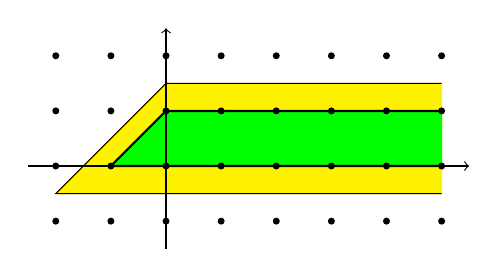
\begin{tikzpicture}[scale=0.7]
	
	\filldraw[yellow] (5,-0.5) -- (-2,-0.5) -- (0,1.5) -- (5,1.5) -- cycle;
	\filldraw[green] (5,0) -- (-1,-0) -- (0,1) -- (5,1) -- cycle;
	
	\foreach \x in {-2,...,5}
	\foreach \y in {-1,...,2}
	{
		\filldraw[fill=black] (\x,\y) circle (1.5pt);
	}
	\draw[->] (-2.5,0) -- (5.5,0);
	\draw[->] (0,-1.5) -- (0,2.5);
	\draw (5,-0.5) -- (-2,-0.5) -- (0,1.5) -- (5,1.5);
	\draw[thick] (5,0) -- (-1,-0) -- (0,1) -- (5,1);
	\end{tikzpicture}
\end{center}

The input is \verb|InhomIneqIH.in| (\verb|InhomIneq.in| augmented by \verb|IntegerHull|). The data of the integer hull are found in \verb|InhomIneqIH.IntHull.out|:
\begin{Verbatim}
...
2 vertices of polyhedron:
-1 0 1
0 1 1

1 extreme rays of recession cone:
1 0 0

3 support hyperplanes of polyhedron (homogenized):
0 -1 1
0  1 0
1 -1 1
\end{Verbatim}

\subsection{Inhomogeneous congruences}\label{ChinRem}

We want to compute the nonnegative solutions of the simultaneous inhomogeneous congruences
\begin{align*}
x_1 + 2x_2 &\equiv 3\pod 7,\\
2x_1 + 2x_2 &\equiv 4\pod{13}
\end{align*}
in two variables. The input file \verb|InhomCong.in| is
\begin{Verbatim}
amb_space 2
constraints 2 symbolic
x[1] + 2x[2] ~ 3 (7);
2x[1] +  2x[2] ~ 4 (13);
\end{Verbatim}
This is an example of input of symbolic constraints. We use \verb|~| as the best ASCII character for representing the congruence sign $\equiv$.

Alternatively one can use a matrix in the input As for which we must move the right hand side over to the left.
\begin{Verbatim}
amb_space 2
inhom_congruences 2
1 2 -3 7
2 2 -4 13
\end{Verbatim}
It is certainly harder to read.

The first vector list in the output:

\begin{Verbatim}
3 module generators:
0 54 1
1  1 1
80  0 1
\end{Verbatim}
Easy to check: if $(1,1)$ is a solution, then it must generate the module of solutions together with the generators of the intersections with the coordinate axes. Perhaps more difficult to find:
\begin{Verbatim}
6 Hilbert basis elements of recession monoid:
0 91 0
1 38 0
3 23 0                                       1 vertices of polyhedron:
5  8 0                                       0 0 91
12  1 0
91  0 0
\end{Verbatim}
Strange, why is $(0,0,1)$, representing the origin in $\RR^2$, not listed as a vertex as well?
Well the vertex shown represents an extreme ray in the lattice $\EE$, and $(0,0,1)$ does not belong to $\EE$.

\begin{Verbatim}
2 extreme rays of recession cone:
0 91 0
91  0 0

3 support hyperplanes of polyhedron (homogenized)
0 0 1
0 1 0
1 0 0

1 congruences:
58 32 1 91
\end{Verbatim}
Normaliz has simplified the system of congruences to a single one.
\begin{Verbatim}
3 basis elements of generated lattice:
1 0  33
0 1 -32
0 0  91
\end{Verbatim}
Again, don't forget that Normaliz prints a basis of the efficient lattice $\EE$.

\subsubsection{Lattice and offset}\label{offset_ex}

The set of solutions to the inhomogeneous system is an affine lattice in $\RR^2$. The lattice basis of $\EE$ above does not immediately let us write down the set of solutions in the form $w+L_0$ with a subgroup $L_0$, but we can easily transform the basis of $\EE$: $(1,1,1)$ is in $\EE$ and we use it to reduce the third column of the other two basis elements to $0$. Try the file \verb|InhomCongLat.in|:

\begin{Verbatim}
amb_space 2
offset
1 1
lattice 2
5 8
-12 -1
\end{Verbatim}


\subsubsection{Variation of the signs}\label{sign_ex}

Suppose we want to solve the system of congruences under the condition that both variables are negative (\verb|InhomCongSigns.in|):

\begin{Verbatim}
amb_space 2
inhom_congruences 2
1 2 -3 7
2 2 -4 13
signs
-1 -1
\end{Verbatim}
The two entries of the sign vector impose the sign conditions $x_1\le 0$ and $x_2\le 0$.

From the output we see that the module generators are more complicated now:
\begin{Verbatim}
4 module generators:
-11   0 1
-4  -7 1
-2 -22 1
0 -37 1
\end{Verbatim}
The Hilbert basis of the recession monoid is simply that of the nonnegative case multiplied by $-1$.

\subsection{Integral closure and Rees algebra of a monomial ideal}\label{Rees}

Next, let us discuss the example \ttt{MonIdeal.in} (typeset in two columns):

\begin{Verbatim}
amb_space 5
rees_algebra 9
1 2 1 2                 1 0 3 4
3 1 1 3                 5 1 0 1
2 5 1 0                 2 4 1 5
0 2 4 3                 2 2 2 4
0 2 3 4
\end{Verbatim}
The input vectors are the exponent vectors of a monomial ideal $I$ in the ring $K[X_1,X_2,X_3,X_4]$. We want to compute the normalization of the Rees algebra of the ideal. In particular we can extract from it the integral closure of the ideal. Since we must introduce an extra variable $T$, we have \verb|amb_space 5|.

In the Hilbert basis we see the exponent vectors of the $X_i$, namely the unit vectors with last component $0$. The vectors with last component $1$ represent the integral closure $\overline I$ of the ideal. There is a vector with last component $2$, showing that the integral closure of $I^2$ is larger than~$\overline I^2$.
\begin{Verbatim}
16 Hilbert basis elements:
0 0 0 1 0
...
5 1 0 1 1
6 5 2 2 2

11 generators of integral closure of the ideal:
0 2 3 4
...
5 1 0 1
\end{Verbatim}
The output of the generators of $\overline I$ is the only place where we suppress the homogenizing variable for ``historic'' reasons. If we extract the vectors with last component $1$ from the extreme rays, then we obtain the smallest monomial ideal that has the same integral closure as $I$.
\begin{Verbatim}
10 extreme rays:
0 0 0 1 0
...
5 1 0 1 1
\end{Verbatim}
The support hyperplanes which are not just sign conditions describe primary decompositions of all the ideals $\overline{I^k}$ by valuation ideals. It is not hard to see that none of them can be omitted for large~$k$ (for example, see: W.~Bruns and G.~Restuccia, Canonical modules of Rees algebras. J.\ Pure Appl.\ Algebra 201, 189--203 (2005)).
\begin{Verbatim}
23 support hyperplanes:
0 0 0  0   1
0 ...
6 0 1  3 -13
\end{Verbatim}

\subsubsection{Only the integral closure of the ideal}

If only the integral closure of the ideal is to be computed, one can choose the input as follows (\verb|IntClMonId.in|):
\begin{Verbatim}
amb_space 4
vertices 9
1 2 1 2 1
...
2 2 2 4 1
cone 4
1 0 0 0
0 1 0 0
0 0 1 0
0 0 0 1
\end{Verbatim}

The generators of the integral closure appear as module generators in the output and the generators of the smallest monomial ideal with this integral closure are the vertices of the polyhedron.



